\documentclass[12pt,aspectratio=169]{beamer}

% ====================================================
% ====================================================
% USEPACKAGES AND IMPORTS
% ====================================================
% ====================================================

\usepackage[T1]{fontenc}
\usepackage[utf8]{inputenc}
\usepackage[english]{babel}

% tables
\usepackage{tabularx}
\usepackage{colortbl}
\usepackage{multirow}
\usepackage{makecell}

% tikz and colors
\usepackage{tikz}
\usepackage{xcolor}
\usepackage{pgfplots}
\usepackage{pgfplotstable}
\usepackage{tikzsymbols}

\usetikzlibrary{calc}
\usetikzlibrary{trees}
\usetikzlibrary{patterns}
\usetikzlibrary{shadings}
\usetikzlibrary{positioning}
\usetikzlibrary{intersections}
\usepgfplotslibrary{patchplots}
\usepgfplotslibrary{fillbetween}
\usetikzlibrary{decorations.pathreplacing}

\usetikzlibrary{arrows}
\usetikzlibrary{arrows.meta}

\usetikzlibrary{shapes}
\usetikzlibrary{shapes.arrows}
\usetikzlibrary{shapes.callouts}
\usetikzlibrary{shapes.symbols}
\usetikzlibrary{shapes.geometric}

% boxes
\usepackage[many]{tcolorbox}

% math packages and fonts
\usepackage{bm}
\usepackage{ccfonts}
\usepackage{eulervm}
\usepackage{amsmath}
\usepackage{amsfonts}
\usepackage{amssymb}
\usepackage{amsthm}
\usepackage{mathtools}
\usepackage{nicefrac}
\usepackage{slashed}
\usepackage{bbold}
\usepackage{array}
\usepackage{cancel}

% algorithms and listings
\usepackage[ruled,vlined,linesnumbered]{algorithm2e}
\usepackage{listings}
\usepackage{setspace}

\tcbuselibrary{listings}
\tcbuselibrary{breakable}
\tcbuselibrary{skins}

% misc
\usepackage{soul}
\usepackage{pifont}
\usepackage{skull}
\usepackage{multicol}
\usepackage{animate}
\usepackage{hyperref}
\usepackage{wasysym}
\usepackage[absolute,overlay]{textpos}
\usepackage[hang,flushmargin]{footmisc}

% ====================================================
% ====================================================
% LAYOUT AND THEME
% ====================================================
% ====================================================

\usetheme{Copenhagen}

% color definitions
\definecolor{myblue1}{RGB}{35,119,189}
\definecolor{myblue2}{RGB}{95,179,238}
\definecolor{myblue3}{RGB}{129,168,207}
\definecolor{myblue4}{RGB}{26,89,142}

\definecolor{myred1}{RGB}{247,12,12}

% set theme colors
\setbeamercolor*{structure}{fg=myblue1,bg=blue}
\setbeamercolor*{palette primary}{use=structure,fg=white,bg=structure.fg}
\setbeamercolor*{palette secondary}{use=structure,fg=white,bg=structure.fg!75!black}
\setbeamercolor*{palette tertiary}{use=structure,fg=white,bg=structure.fg!50!black}
\setbeamercolor*{palette quaternary}{fg=black,bg=white}

\setbeamertemplate{itemize item}[circle]
\setbeamertemplate{itemize subitem}[circle]
\setbeamertemplate{itemize subsubitem}[circle]

\setbeamertemplate{enumerate item}[circle]
\setbeamertemplate{enumerate subitem}[circle]
\setbeamertemplate{enumerate subsubitem}[circle]

\setbeamercolor{itemize item}{fg=myblue1}
\setbeamercolor{itemize subitem}{fg=myblue1}
\setbeamercolor{itemize subsubitem}{fg=myblue1}

\setbeamertemplate{section in toc}[circle]
\setbeamertemplate{subsection in toc}[circle]
\setbeamerfont{subsection in toc}{size=\scriptsize}

\setbeamercolor{frametitle continuation}{fg=black}

% title graphic -- sap logo and dhbw logo
\titlegraphic{
\includegraphics[scale=0.1]{../03_img/logo_sap}\hspace*{4.75cm}~%
   	
\includegraphics[scale=0.05]{../03_img/logo_dhbw}
}

\makeatletter
% frame title
\defbeamertemplate*{frametitle}{mydefault}[1][left]
{
  	\ifbeamercolorempty[bg]{frametitle}{}{\nointerlineskip}%
  	\nointerlineskip%
 	\@tempdima=\textwidth%
  	\advance\@tempdima by\beamer@leftmargin%
  	\advance\@tempdima by\beamer@rightmargin%
  	\begin{tcolorbox}[
  		enhanced,
  		outer arc=0pt,
  		arc=0pt,
  		boxrule=0pt,
  		top=0pt,
  		bottom=0pt,
  		enlarge left by=-\beamer@leftmargin,
  		enlarge right by=-\beamer@rightmargin,
  		width=\paperwidth,
  		nobeforeafter,
  		interior style={
    			left color=myblue2,
    			right color=white
    		},
  		shadow={0mm}{-0.4mm}{0mm}{black!60,opacity=0.6},    
  		shadow={0mm}{-0.8mm}{0mm}{black!40,opacity=0.4},    
  	]
    	\usebeamerfont{frametitle}%
    	\vbox{}\vskip-1ex%
    	\if@tempswa\else\csname beamer@fte#1\endcsname\fi%
    	\insertframetitle\par%
    	{%
      		\ifx\insertframesubtitle\@empty%
      		\else%
      		{\usebeamerfont{framesubtitle}\usebeamercolor[fg]{black}\insertframesubtitle\strut\par}%
      		\fi
    	}%
    	\vskip-1ex%
    	\if@tempswa\else\vskip-.3cm\fi
  	\end{tcolorbox}%
}

% footline of a frame
\defbeamertemplate*{footline}{mysplit theme}
{%
  	\leavevmode%
  	\hbox{
		\begin{beamercolorbox}[
			wd=.5\paperwidth,ht=2.5ex,dp=1.125ex,leftskip=.3cm plus1fill,rightskip=.3cm
		]{author in head/foot}%
    			\usebeamerfont{author in head/foot}\insertshortauthor\ (\insertinstitute), \insertdate
  		\end{beamercolorbox}%
  		\begin{beamercolorbox}[
			wd=.5\paperwidth,ht=2.5ex,dp=1.125ex,leftskip=.3cm,rightskip=.3cm plus1fil
		]{title in head/foot}%
    			\usebeamerfont{title in head/foot}\insertshorttitle\hfill
    			\insertprefix-\insertframenumber/\inserttotalframenumber\hspace*{0.5em}
  		\end{beamercolorbox}}%
  	\vskip0pt%
}
\makeatother

% ====================================================
% ====================================================
% COMMANDS AND GENERAL DEFINITIONS
% ====================================================
% ====================================================

% page number prefix
\newcommand\insertprefix{}  % empty by default
\newcommand\prefix[1]{\renewcommand\insertprefix{#1}}

% math definitions
% ====================================================
\DeclareMathOperator*{\argmax}{arg\,max}
\DeclareMathOperator*{\argmin}{arg\,min}
\newcommand*\diff{\mathop{}\!\mathrm{d}}

\newcommand*{\vertbar}{\rule[-1ex]{0.5pt}{2.5ex}}
\newcommand*{\horzbar}{\rule[.5ex]{2.5ex}{0.5pt}}

% commands
% ====================================================

% highlight commands
% --------------------------------------------------------------------------------------------------------
% highlight command
\newcommand{\highlight}[1]{\textcolor{myblue1}{\textbf{#1}}}
\newcommand{\highlighttt}[1]{\textcolor{myblue1}{\texttt{#1}}}
\newcommand{\Highlight}[1]{\textcolor{myred1}{\textbf{#1}}}

% blue color boxes (with frame/without frame/without fill)
\newtcolorbox{boxBlue}{colback=myblue1!10!white,colframe=myblue4}
\newtcolorbox{boxBlueNoFrame}{colback=myblue1!10!white,colframe=myblue1!10!white}
\newtcolorbox{boxBlueNoFill}{colback=white,colframe=myblue4}

% font commands
% --------------------------------------------------------------------------------------------------------
\newcommand{\linkstyle}[1]{\underline{\smash{\texttt{#1}}}} 		% style of hyperlinks

% tikz commands
% --------------------------------------------------------------------------------------------------------

% yellow sticky note
\newcommand{\bubble}[3]{
\begin{textblock}{100}(#1, #2)
      	\begin{tikzpicture}
		\node[rectangle,draw=yellow,very thick,fill=yellow!60,align=center] at (0,0) {#3};
	\end{tikzpicture}
\end{textblock}
}

\newcommand{\floattext}[3]{
\begin{textblock}{100}(#1, #2)
      	#3
\end{textblock}
}

\newcommand{\doublecircle}[2]{
	\draw[fill=white,draw=myblue1] (#1,#2) circle (2mm);
	\draw[fill=myblue1,draw=myblue1] (#1,#2) circle (1.5mm);
}

% slide modifiers
% --------------------------------------------------------------------------------------------------------
% mark slide as optional
\newcommand{\optional}{
	\begin{textblock}{100}(0.15,0.30)
      		
\includegraphics[scale=0.2]{../03_img/scream}
    	\end{textblock}
}

% mark slide as important
\newcommand{\important}{
	\begin{textblock}{100}(0.10,0.15)
      		
\includegraphics[scale=0.1]{../03_img/important}
    	\end{textblock}
}

% citation
% --------------------------------------------------------------------------------------------------------
% first argument in {book, online, article}
\newcommand{\literature}[5]{
	\setbeamertemplate{bibliography item}[#1]
	\bibitem{#2}
	\highlight{#3} \\
	\textcolor{darkgray}{\textit{#4}} \\
	\textcolor{black}{#5}
}
% cite content
\newcommand{\citeAuthor}[3]{\vfill\scriptsize\textcolor{lightgray}{#1 \cite{#2} #3}}

% slide architecture
% --------------------------------------------------------------------------------------------------------
% divide frame into two parts
\newcommand{\divideTwo}[4]{
	\begin{minipage}{#1\textwidth}
		#2
	\end{minipage}
	\hfill
	\begin{minipage}{#3\textwidth}
		#4
	\end{minipage}
}

% divide frame into two parts (start on top)
\newcommand{\divideTwoTop}[4]{
	\begin{minipage}[t]{#1\textwidth}
		#2
	\end{minipage}
	\hfill
	\begin{minipage}[t]{#3\textwidth}
		#4
	\end{minipage}
}

% special pages
% --------------------------------------------------------------------------------------------------------
% title page
\newcommand{\maketitlepage}{
	{
		\beamertemplatenavigationsymbolsempty
		\usebackgroundtemplate{%
			\tikz[overlay,remember picture] \node[opacity=0.2, at=(current page.center)] {
  				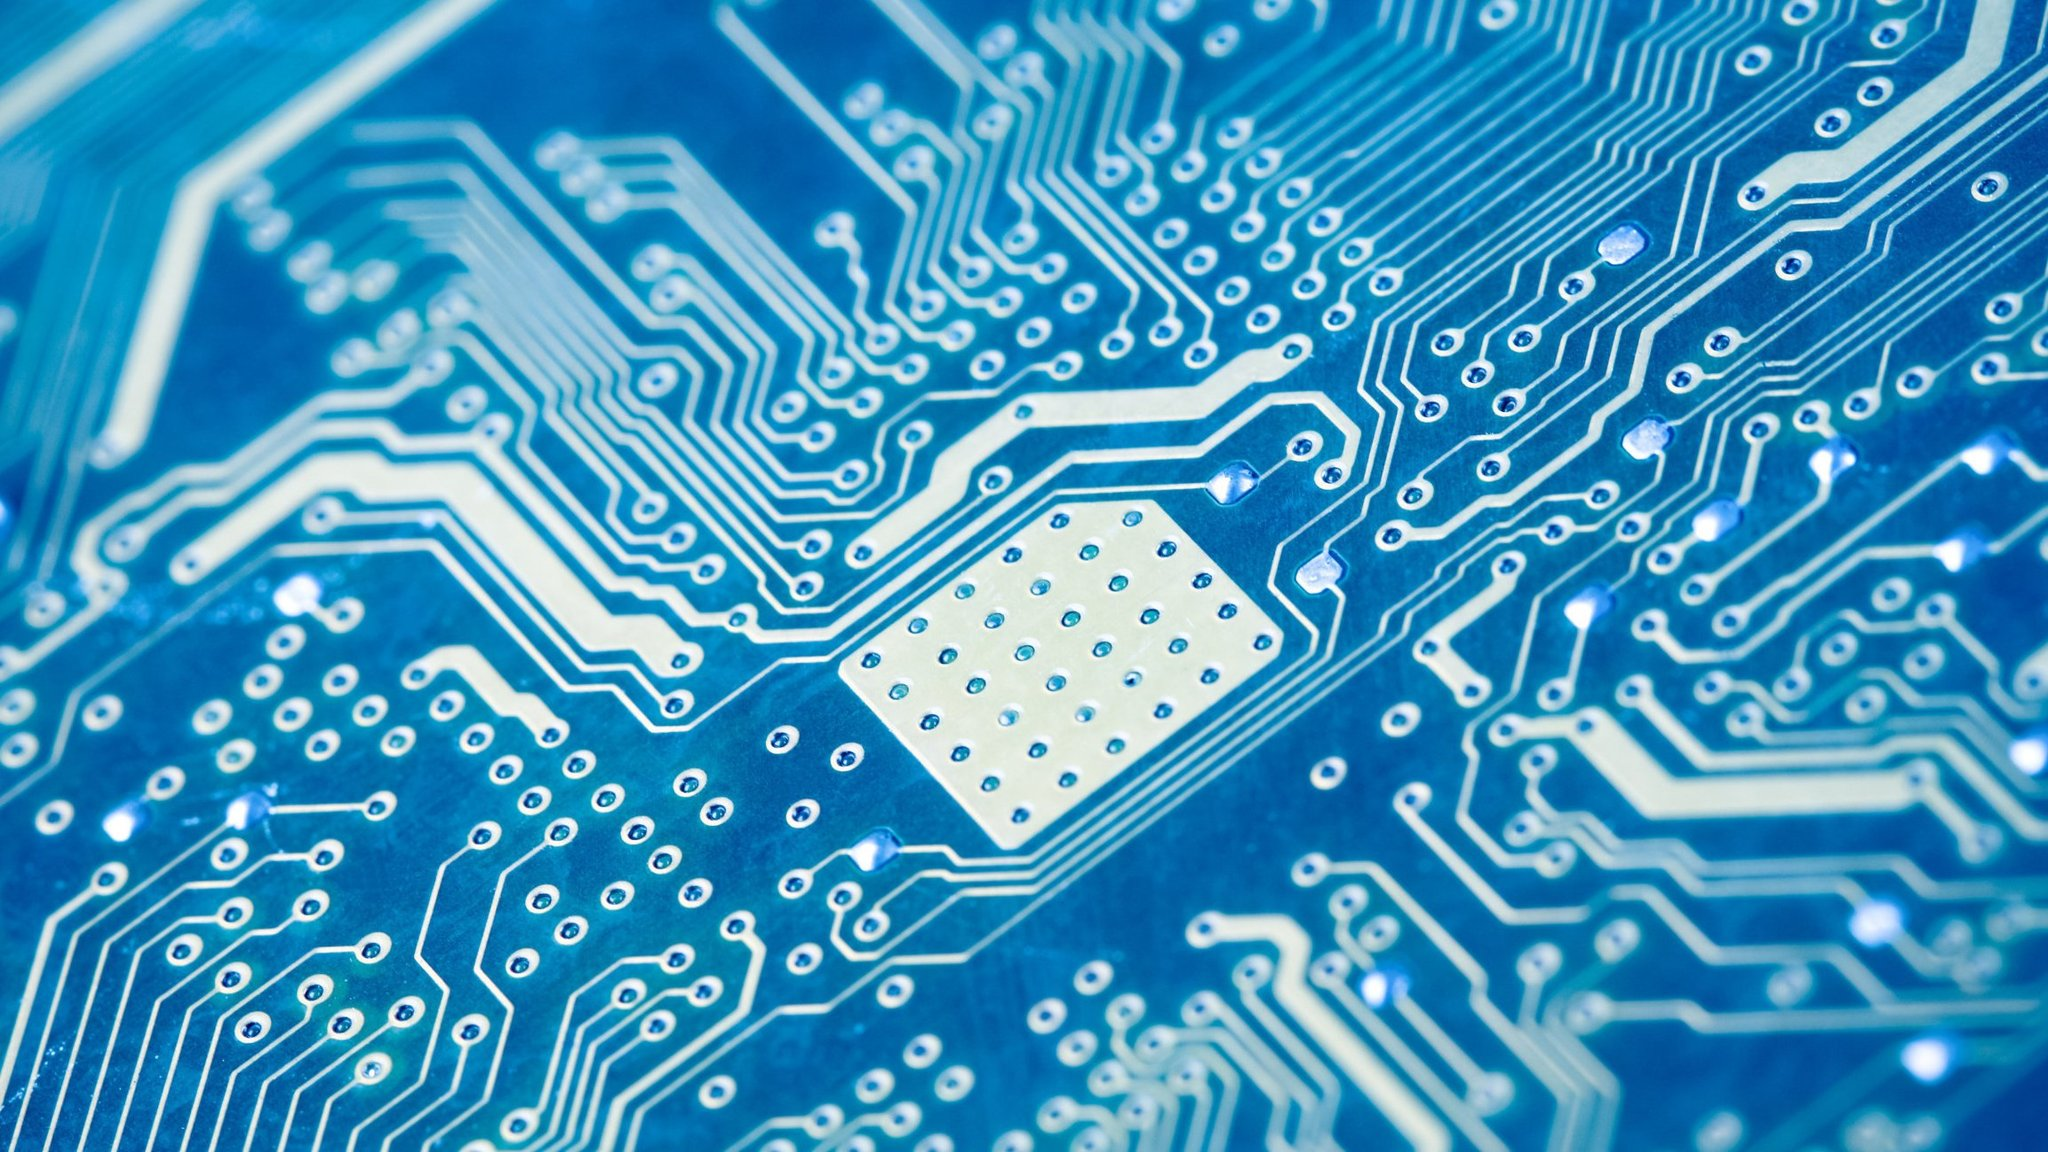
\includegraphics[height=\paperheight,width=\paperwidth]{../03_img/processor.jpg}
			};
		}
		\begin{frame}[plain]
			\vspace*{0.75cm}
			\maketitle
			\vfill
			\begin{center}
				\footnotesize Find all slides on \href{https://github.com/DaWe1992/Applied_ML_Fundamentals}{\linkstyle{GitHub}}
			\end{center}
		\end{frame}
	}
}

% divider page
\newcommand{\makedivider}[1]{
	{
		\beamertemplatenavigationsymbolsempty
		\usebackgroundtemplate{%
			\tikz[overlay,remember picture] \node[opacity=0.2, at=(current page.center)] {
  				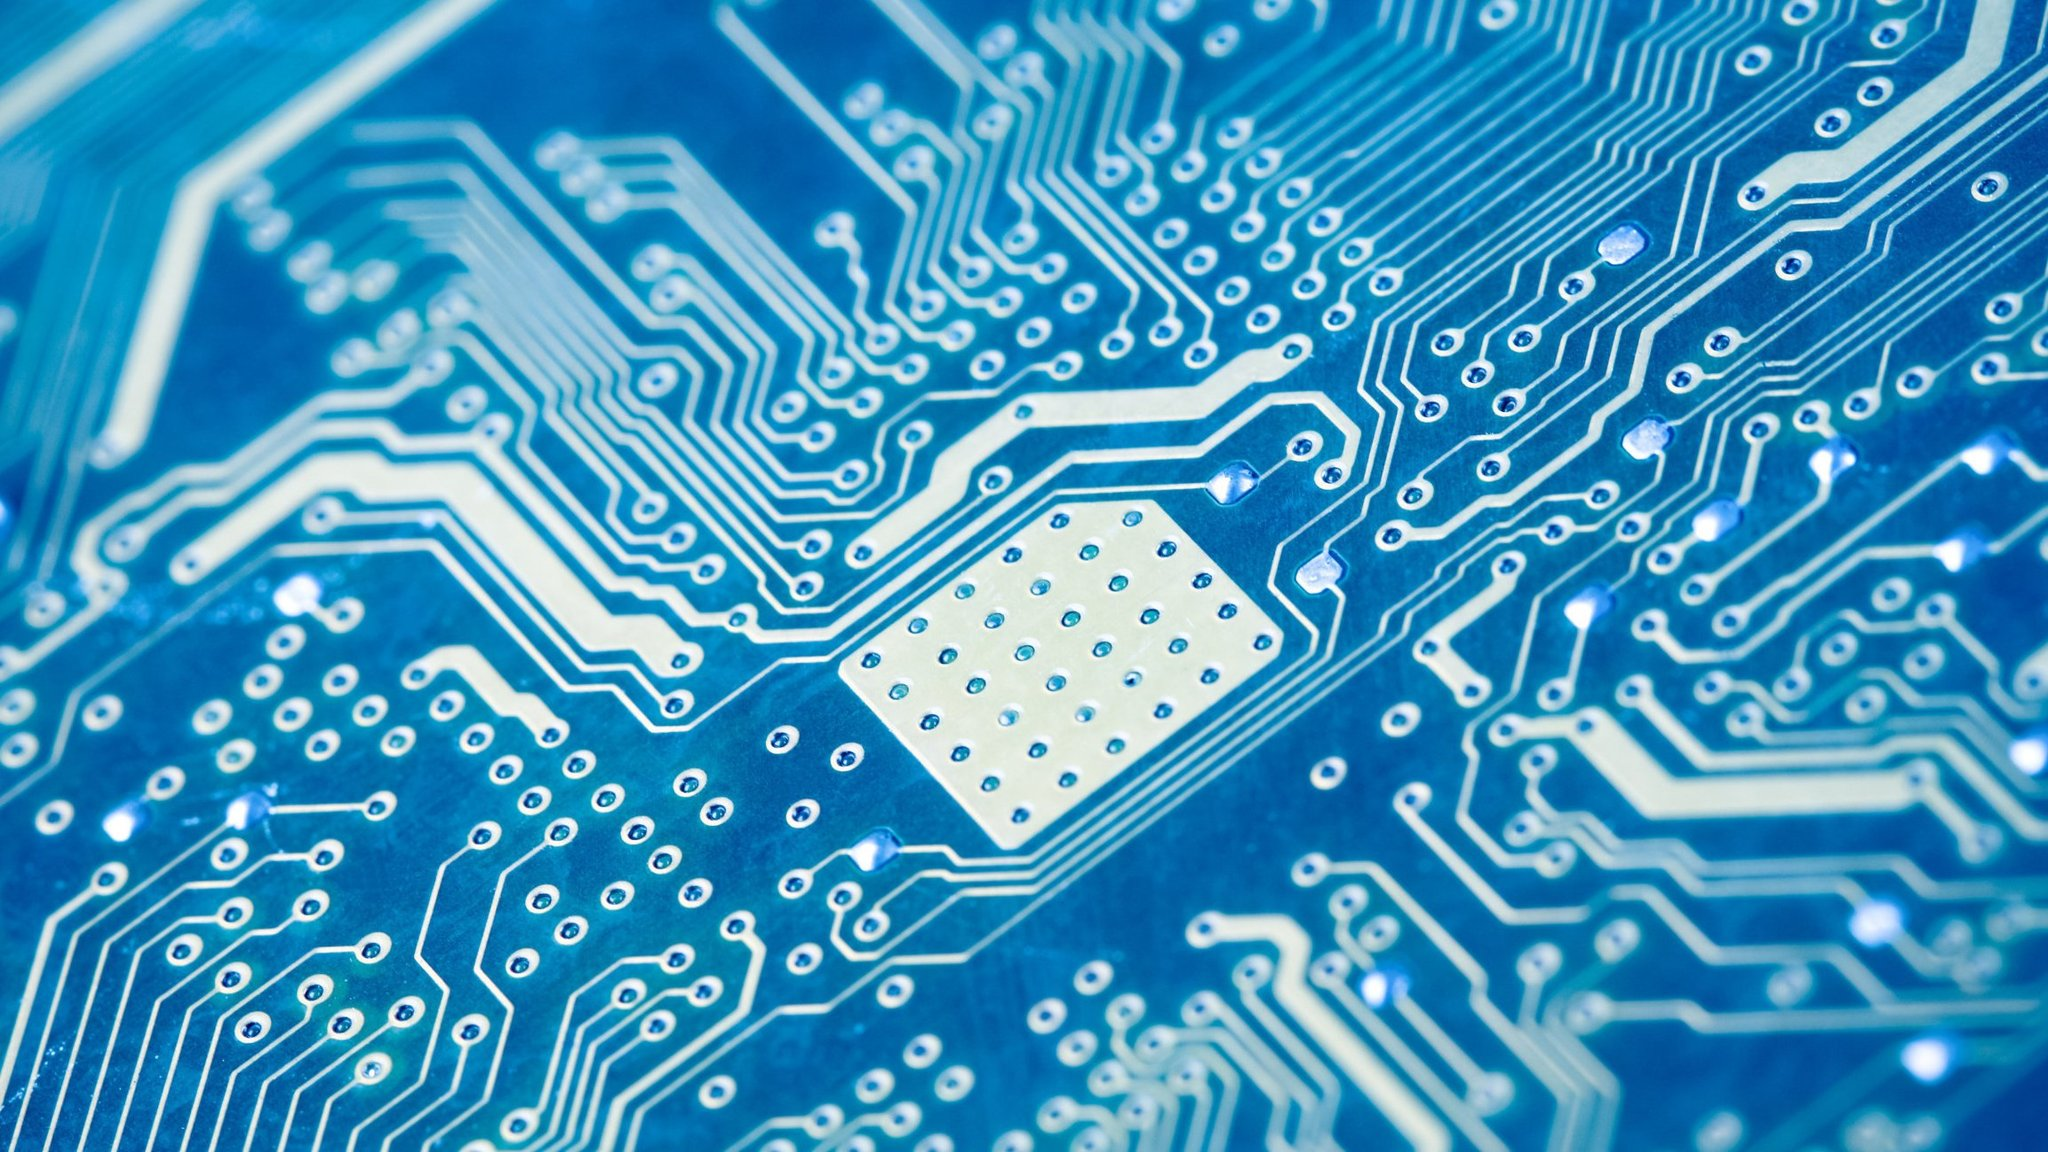
\includegraphics[height=\paperheight,width=\paperwidth]{../03_img/processor.jpg}
			};
		}
		\begin{frame}[plain]
			\vfill
			\begin{boxBlue}
				\centering
				\textbf{Section:} \\
				\large \highlight{#1}
			\end{boxBlue}
			\vfill
			\centering
			
\includegraphics[scale=0.05]{../03_img/logo_dhbw.png}
			\vfill
		\end{frame}
	}
}

% overview page
\newcommand{\makeoverview}[1]{
	\begin{frame}{Lecture Overview}{}
		\begin{tabbing}
			\hspace*{3.5cm}\= \kill
			\ifnum #1=1 \highlight{\textbf{Unit I:}} \else \textbf{Unit I:} \fi
			\> \ifnum #1=1 \highlight{Machine Learning Introduction} \else Machine Learning Introduction \fi \\
		\end{tabbing}
	\end{frame}
}

% thank you page
\newcommand{\makethanks}{
	{\beamertemplatenavigationsymbolsempty
	\begin{frame}[plain]
		\vfill
		\begin{boxBlue}
			\centering
			\Large \highlight{Thank you very much for the attention!}
		\end{boxBlue}
		
		\vfill\footnotesize
		\begin{tabbing}
			\hspace*{1.5cm}\= \kill
			\highlight{Topic:} 	\> \inserttitle \\
			\highlight{Date:} 	\> \insertdate
		\end{tabbing}
		
		\vfill
		\highlight{Contact:} \\
		\insertauthor\ (D062271) \\
		\insertinstitute \\
		\href{mailto:daniel.wehner@sap.com}{\linkstyle{daniel.wehner@sap.com}}
		
		\vfill\normalsize
		\begin{center}
			\large\highlight{Do you have any questions?}
		\end{center}
		\vfill
	\end{frame}}
}

% global pfgplots settings
% --------------------------------------------------------------------------------------------------------
\pgfplotsset{
	% allow filtering of data for pgfplots
	discard if/.style 2 args={
        		x filter/.code={
            		\edef\tempa{\thisrow{#1}}
            		\edef\tempb{#2}
            		\ifx\tempa\tempb
                		\def\pgfmathresult{inf}
            		\fi
        		}
    	},
    	discard if not/.style 2 args={
        		x filter/.code={
            		\edef\tempa{\thisrow{#1}}
            		\edef\tempb{#2}
            		\ifx\tempa\tempb
            		\else
                		\def\pgfmathresult{inf}
            		\fi
        		}
    	}
}


% ====================================================
% ====================================================
% PRESENTATION DATA
% ====================================================
% ====================================================

\title[Evaluation of ML Models]{*** Applied Machine Learning Fundamentals *** Evaluation of ML Models}
\institute[SAP\,SE]{SAP\,SE / DHBW Mannheim}
\author{Daniel Wehner, M.Sc.}
\date{Winter term 2022/2023}
\prefix{EVAL}

% ====================================================
% ====================================================
% BEGIN OF DOCUMENT
% ====================================================
% ====================================================

\begin{document}

% Title frame
%______________________________________________________________________
\maketitlepage


% Lecture Overview
%______________________________________________________________________
\begin{frame}{Lecture Overview}{}
	\makeoverview{7}
\end{frame}


% Agenda
%______________________________________________________________________
\begin{frame}{Agenda for this Unit}
	\begin{multicols}{2}
		\tableofcontents
	\end{multicols}
\end{frame}


% Section: Evaluation Methods and Data Splits
%______________________________________________________________________
\section{Evaluation Methods and Data Splits}
\makedivider{Evaluation Methods and Data Splits}

% Subsection: Introduction
% --------------------------------------------------------------------------------------------------------
\subsection{Introduction}

% Evaluation of trained Models
\begin{frame}{Evaluation of trained Models}{}
	\begin{enumerate}
		\item \highlight{Validation through experts}: A domain expert checks plausibility
		\begin{itemize}
			\item Subjective, time-intensive, costly
			\item Often the only option
		\end{itemize}
		\item \highlight{Validation on data}: Evaluate performance on a \textbf{separate (!)} test set
		\begin{itemize}
			\item Labeled data is scarce, could be better used for training
			\item Fast and simple, no domain knowledge needed
		\end{itemize}
		\item \highlight{On-line validation}: Test model in a fielded application
		\begin{itemize}
			\item Bad models may be costly
			\item Gives the best estimate for the overall utility
		\end{itemize}
	\end{enumerate}
\end{frame}


% Out-of-Sample Testing
\begin{frame}{Out-of-Sample Testing}{}\important
	\begin{itemize}
		\item The performance cannot be measured on the training data ($\Rightarrow$ overfitting!)
		\item Usually, a portion of the available data is reserved for testing
		\begin{itemize}
			\item $\nicefrac{2}{3}$ for training, $\nicefrac{1}{3}$ for testing (evaluation)
			\item The model is trained on the training set and evaluated on the test set
		\end{itemize}
		\item \textbf{Problems}:
		\begin{itemize}
			\item Waste of data
			\item Labeling may be expensive
		\end{itemize}
		\item \textbf{Solution}: \highlight{Cross-Validation (X-Val)}
	\end{itemize}
\end{frame}


% Subsection: Cross-Validation / LOO-Validation
% --------------------------------------------------------------------------------------------------------
\subsection{Cross-Validation / LOO-Validation}

% Cross-Validation (X-Val)
\begin{frame}{Cross-Validation (X-Val)}{}\important
	\begin{itemize}
		\item Split the data set into $k$ equally sized partitions $P = \{ p_1, p_2, \dots, p_k \}$
		\item \texttt{For each} partition $p_i$ \texttt{do}: use $p_i$ for testing and $P \backslash \{ p_i \}$ for training
		\item Average the results; e.\,g. 4-fold X-Val:
	\end{itemize}
	
	\vspace*{-3mm}
	\begin{figure}
	\centering
	\begin{tikzpicture}[
		scale=0.8
	]
	
		\foreach \y/\x/\p in {1/6/$p_4$,2/4/$p_3$,3/2/$p_2$,4/0/$p_1$}{
			\fill[myblue1] (\x,\y) -- (\x+2,\y) -- (\x+2,\y+0.5) -- (\x,\y+0.5) -- cycle;
			\draw (0,\y) -- (8,\y) -- (8,\y+0.5) -- (0,\y+0.5) -- cycle;
			\draw (2,\y) -- (2,\y+0.5);
			\draw (4,\y) -- (4,\y+0.5);
			\draw (6,\y) -- (6,\y+0.5);
			\node at(\x+1,4.75) {\footnotesize \p};
		}
		
	\end{tikzpicture}
\end{figure}
\end{frame}


% Leave-One-Out Cross-Validation (LOO X-Val)
\begin{frame}{Leave-One-Out Cross-Validation (LOO X-Val)}{}
	\vspace*{2mm}
	\divideTwo{0.49}{
		\begin{itemize}
			\item $n$-fold X-Val
			\begin{itemize}
				\item $n$ is the number of examples
				\item Use $n - 1$ examples for training, one example for testing
			\end{itemize}
		\end{itemize}
	}{0.49}{
		\begin{itemize}
			\item Properties
			\begin{itemize}
				\item Makes best use of the data
				\item Very expensive for large data sets (large $n$)
			\end{itemize}
		\end{itemize}
	}
	
	\vspace*{3mm}
	\begin{boxBlueNoFrame}
		\highlight{If $k$-fold X-Val is performed, we get $k$ trained models!}
		
	\end{boxBlueNoFrame}
	
	\begin{itemize}
		\item \textbf{Which model is used in production?}
		\item \textbf{Answer:} None. X-Val is only used for error estimation. The final model is trained on the entire data set
	\end{itemize}
\end{frame}


% Subsection: Data Splits
% --------------------------------------------------------------------------------------------------------
\subsection{Data Splits}

% Three Splits: Train, Dev/Validation, Test
\begin{frame}{Three Splits: Train, Dev/Validation, Test}{}\important
	\bubble{10.25}{5.5}{
		\footnotesize \highlight{Stratified splits} have the same \\[-1mm]
		\footnotesize class dist. as the entire data set
	}
	In practice it is common to split the data into three portions:
	\vspace*{3mm}
	\begin{boxBlueNoFrame}
		\begin{enumerate}
			\item \highlight{Training set} {\footnotesize (used for training as before)}
			\item \highlight{Dev/Validation set}
			\begin{itemize}
				\item Used for hyper-parameter tuning of the model
				\item Using the test set for that would be cheating
			\end{itemize}
			\item \highlight{Test set}
			\begin{itemize}
				\item The final model is tested on the test set
				\item Test set is used to estimate the \textbf{generalization error}
			\end{itemize}
		\end{enumerate}
	\end{boxBlueNoFrame}
\end{frame}


% Section: Evaluation Metrics
%______________________________________________________________________
\section{Evaluation Metrics}
\makedivider{Evaluation Metrics}

% Subsection: Confusion Matrices
% --------------------------------------------------------------------------------------------------------
\subsection{Confusion Matrices}

% Types of Errors
\begin{frame}{Types of Errors}{}
	\bubble{12}{6}{\footnotesize a.\,k.\,a. $\alpha/\beta$ error}
	\begin{itemize}
		\item \highlight{Type I Error}: False negatives
		\begin{itemize}
			\item An instance which is labeled $\oplus$ is classified as $\ominus$
			\item E.\,g. a spam e-mail is not detected
		\end{itemize}
		\item \highlight{Type II Error}: False positives
		\begin{itemize}
			\item An instance which is labeled $\ominus$ is classified as $\oplus$
			\item E.\,g. a non-spam (ham) e-mail is classified as spam
		\end{itemize}
	\end{itemize}
	
	\vspace*{2mm}
	\begin{boxBlueNoFrame}
		\highlight{Depending on the context the costs of false negatives and false positives can be different!}
	\end{boxBlueNoFrame}
\end{frame}


% Confusion Matrices (two Classes)
\begin{frame}{Confusion Matrices (two Classes)}{}\important
	\vspace*{2mm}
	\begin{itemize}
		\item How often is class $\mathcal{C}_i$ confused with class $\mathcal{C}_j$?
		\item Calculate \highlight{accuracy}:
	\end{itemize}
	\begin{table}[h]
	\scalebox{0.8}{
	\begin{tabular}{| c | c | c |}
		\hline
		\rowcolor{lightgray}
 		&
		\textbf{Classified} $\bm{\oplus}$ &
		\textbf{Classified} $\bm{\ominus}$
		\\ \hline
		\cellcolor{lightgray}\textbf{Is} $\bm{\oplus}$ 
			& \textcolor{myblue1}{true positives ($tp$)} 
			& false negatives ($fn$)
		\\ \hline
		\cellcolor{lightgray}\textbf{Is} $\bm{\ominus}$ 
			& false positives ($fp$) 
			& \textcolor{myblue1}{true negatives ($tn$)}
		\\ \hline
	\end{tabular}}
\end{table}
	\vspace*{-5mm}
	\begin{align*}
		accuracy 	&= \frac{tp + tn}{tp + tn + fp + fn} \\[3mm]
		error		&= 1 - accuracy
	\end{align*}
\end{frame}


% Confusion Matrices (multiple Classes)
\begin{frame}{Confusion Matrices (multiple Classes)}{}
	\begin{table}[h]
	\scalebox{1.0}{
	\begin{tabular}{| c | c | c | c | c | c |}
		\hline
		\rowcolor{lightgray}
 		&
		\textbf{A} &
		\textbf{B} &
		\textbf{C} &
		\textbf{D} &
		$\bm{\Sigma}$
		\\ \hline\hline
		\cellcolor{lightgray}
		\textbf{A} 		&	$\textcolor{myblue1}{n_{A,A}}$ 	&	$n_{B,A}$	 					&	$n_{C,A}$	 				&	$n_{D,A}$ 					&	\cellcolor{lightgray}$n_{A}$ 	\\ \hline
		\cellcolor{lightgray}
		\textbf{B} 		&	$n_{A,B}$ 				&	$\textcolor{myblue1}{n_{B,B}}$	 	&	$n_{C,B}$	 				&	$n_{D,B}$ 					&	\cellcolor{lightgray}$n_{B}$ 	\\ \hline
		\cellcolor{lightgray}
		\textbf{C} 		&	$n_{A,C}$ 				&	$n_{B,C}$	 					&	$\textcolor{myblue1}{n_{C,C}}$	 &	$n_{D,C}$ 					&	\cellcolor{lightgray}$n_{C}$ 	\\ \hline
		\cellcolor{lightgray}
		\textbf{D} 		&	$n_{A,D}$ 				&	$n_{B,D}$	 					& 	$n_{C,D}$					 &	$\textcolor{myblue1}{n_{D,D}}$ 	&	\cellcolor{lightgray}$n_{D}$ 	\\ \hline\hline
		\rowcolor{lightgray}
		$\bm{\Sigma}$	&	$\overline{n_A}$
					& 	$\overline{n_B}$
					& 	$\overline{n_C}$
					& 	$\overline{n_D}$
					& 	$n$ 				\\ \hline
	\end{tabular}}
\end{table}
	
	\vspace*{2mm}
	\begin{equation*}
		accuracy = \frac{n_{A,A} + n_{B,B} + n_{C,C} + n_{D,D}}{n}
	\end{equation*}
\end{frame}


% Subsection: Drawback of Accuracy
% --------------------------------------------------------------------------------------------------------
\subsection{Drawback of Accuracy}

% Drawback of Accuracy
\begin{frame}{Drawback of Accuracy}{}
	\begin{itemize}
		\item Real-world data sets are usually \textbf{imbalanced}, i.\,e. some classes appear more frequently than others
		\item \textbf{Example}:
		\begin{itemize}
			\item A data set $\mathcal{D}$ contains two classes $\mathcal{C}_1$ and $\mathcal{C}_2$
			\item $\mathcal{C}_1$ appears 99\,\% of the time, $\mathcal{C}_2$ 1\,\% of the time
			\item It is easy to reach 99\,\% accuracy by always predicting the majority class
			\item \textbf{Is this useful?} \textit{Probably not...}
		\end{itemize}
	\end{itemize}
	
	\vspace*{2mm}
	\begin{boxBlueNoFrame}
		\textbf{We need some more sophisticated evaluation metrics!}
	\end{boxBlueNoFrame}
\end{frame}


% Subsection: Precision, Recall and F1-Score
% --------------------------------------------------------------------------------------------------------
\subsection{Precision, Recall and F1-Score}

% Precision and Recall
\begin{frame}{Precision and Recall}{}\important
	\begin{boxBlueNoFrame}
		\highlight{Precision}: Ratio of $tp$ to all instances predicted as $\oplus$
		\begin{equation}
			Precision\ (P) = \frac{tp}{tp + fp}
		\end{equation}
	\end{boxBlueNoFrame}

	\begin{boxBlueNoFrame}
		\highlight{Recall} (Sensitivity): Ratio of $tp$ to all instances actually labeled as $\oplus$
		\begin{equation}
			Recall\ (R) = \frac{tp}{tp + fn}
		\end{equation}
	\end{boxBlueNoFrame}
\end{frame}


% Precision-Recall-Trade-Off
\begin{frame}{Precision-Recall-Trade-Off}{}
	\vspace*{-4mm}
	\begin{center}
		\highlight{There is a trade-off between precision and recall:}
	\end{center}
	\vspace*{-3mm}
	\begin{boxBlueNoFrame}
		\textbf{It is very easy to get 100\,\% precision:}
		\begin{itemize}
			\item Simply classify one instance as $\oplus$ where you are absolutely sure
			\item But recall is bad... {\footnotesize \textit{(many $\oplus$-instances are not detected)}}
		\end{itemize}
		\vspace*{2mm}
		\hrule
		\vspace*{2mm}
		\textbf{It is also quite easy to achieve 100\,\% recall:}
		\begin{itemize}
			\item Classify all instances as $\oplus$
			\item But precision is bad... {\footnotesize \textit{(many $\ominus$-instances are detected)}}
		\end{itemize}
	\end{boxBlueNoFrame}
\end{frame}


% Precision-Recall Curves / P-R-Curves
\begin{frame}{Precision-Recall Curves / P-R-Curves}{}
	\begin{itemize}
		\item Visualization of the Precision-Recall-trade-off
		\item Influence precision and recall by changing thresholds
		\item \textbf{Example}:
		\begin{itemize}
			\item Consider a ranker, e.\,g. a logistic regression classifier
			\item It outputs probabilities for each class
			\item The threshold when to predict $\oplus$ can be changed
			\item This has an influence on precision and recall
		\end{itemize}
	\end{itemize}
	
	\vspace*{2mm}
	\begin{boxBlueNoFrame}
		\highlight{A P-R-curve plots precision and recall for all possible thresholds.}
	\end{boxBlueNoFrame}
\end{frame}


% Precision-Recall Curves / P-R-Curves (Ctd.)
\begin{frame}{Precision-Recall Curves / P-R-Curves (Ctd.)}{}
	\begin{figure}
	\centering
	\begin{tikzpicture}[
		scale=0.9
	]

		\begin{axis}[
			grid=both,
    			grid style={line width=.1pt, draw=gray!10},
			xlabel={\footnotesize{\textbf{Recall}}},
			ylabel={\footnotesize{\textbf{Precision}}},
			y=8cm,
    			x=8cm,
			legend pos= south west
		]
	
    			\pgfplotstableread{09_evaluation/05_data/p_r_curve_svm.txt} \datatable
			\addplot[no marks,myblue1,very thick] table[x=r,y=p] from \datatable;
			\addplot[mark=o,mark size=5pt,myblue1] plot coordinates {(0.869281045751634, 0.8471337579617835)};

			\pgfplotstableread{09_evaluation/05_data/p_r_curve_rf.txt} \datatable
			\addplot[no marks,gray,very thick] table[x=r,y=p] from \datatable;
			\addplot[mark=o,mark size=5pt,gray] plot coordinates {(0.8954248366013072, 0.8954248366013072)};

			\legend{svm, threshold 0 svm, rf, threshold 0.5 rf}
			
    		\end{axis}
		
	\end{tikzpicture}
\end{figure}
\end{frame}


% Combining Precision and Recall: F1-Score
\begin{frame}{Combining Precision and Recall: F1-Score}{}\important
	\bubble{10.5}{6.5}{\footnotesize Why the harmonic mean?}
	\begin{itemize}
		\item When to use precision, when recall?
		\item This depends on the cost of $fp$ and $fn$
		\begin{itemize}
			\item If $fp$ are expensive $\Rightarrow$ \textbf{use precision!}
			\item If $fn$ are expensive $\Rightarrow$ \textbf{use recall!}
		\end{itemize}
		\item \highlight{F1-score} \textit{(harmonic mean of precision and recall)}
		\begin{equation}
			F_1 = \frac{2 \cdot P \cdot R}{P + R} \qquad\quad
			F_{\beta} = (1 + \beta^2) \cdot \frac{P \cdot R}{(\beta^2 \cdot P) + R} \quad (\beta \in \mathbb{R}^+)
		\end{equation}
		\item Large $\beta$ emphasizes recall
	\end{itemize}
\end{frame}


% Calculation for multiple Classes (Example Precision)
\begin{frame}{Calculation for multiple Classes (Example Precision)}{}
	\begin{itemize}
		\item Precision must be calculated for each class separately
		\item For $\vert \mathcal{C} \vert$ classes we get $\vert \mathcal{C} \vert$ results. \textbf{How to combine?}
		\begin{itemize}
			\item \highlight{Macro average:} Calculate $P$ for each class and average the result
			\begin{equation}
				P_{macro} = \frac{P_A + P_B + P_C + P_D}{\vert \mathcal{C} \vert}
			\end{equation}
			\item \highlight{Micro average:} Sum all $tp$ and $fp$ for all classes and calculate $P$
			\begin{equation}
				P_{micro} = \frac{tp_A + tp_B + tp_C + tp_D}{(tp_A + tp_B + tp_C + tp_D) + (fp_A + fp_B + fp_C + fp_D)}
			\end{equation}
		\end{itemize}
	\end{itemize}
\end{frame}


% Calculation for multiple Classes (Example Precision)
\begin{frame}{Calculation for multiple Classes (Example Precision)}{}
	\bubble{2.5}{12}{
		\footnotesize Cols: Prediction \\[-1mm]
		\footnotesize Rows: Gold label
	}
	\divideTwo{0.39}{
		\begin{table}[h]
	\scalebox{0.8}{
	\begin{tabular}{| c | c | c | c | c | c |}
		\hline
		\rowcolor{lightgray}
 		&
		\textbf{A} &
		\textbf{B} &
		\textbf{C} &
		\textbf{D} &
		$\bm{\Sigma}$
																	\\ \hline\hline
		\cellcolor{lightgray} \textbf{A}	& 40 & 12 & 4 	& 8 	& \cellcolor{lightgray} 64 	\\ \hline	
		\cellcolor{lightgray} \textbf{B} 	& 7 	& 51 & 2 	& 0 	& \cellcolor{lightgray} 60 	\\ \hline	
		\cellcolor{lightgray} \textbf{C} 	& 2 	& 17 & 27 & 11 & \cellcolor{lightgray} 57 	\\ \hline	
		\cellcolor{lightgray} \textbf{D} 	& 39 & 4	& 15 & 8	& \cellcolor{lightgray} 66 	\\ \hline\hline
		\rowcolor{lightgray}
		$\bm{\Sigma}$				& 88 & 84 & 48 & 27 & \cellcolor{lightgray} 247	\\ \hline
	\end{tabular}}
\end{table}
	}{0.59}{
		\begin{align*}
			P_A 			&= \frac{40}{40 + 48} = 0.45 							\\[0.5mm]
			P_B 			&= 0.61											\\[0.5mm]
			P_C 			&= 0.56											\\[0.5mm]
			P_D 			&= 0.30											\\[0.5mm]
			P_{macro} 	&= \frac{0.45 + 0.61 + 0.56 + 0.30}{4} = 0.48 				\\[0.5mm]
			P_{micro}		&= \frac{40 + ... + 8}{(40 + ... + 8) + (48 + ... + 19)} = 0.51
		\end{align*}
	}
\end{frame}


% Subsection: ROC and AUC
% --------------------------------------------------------------------------------------------------------
\subsection{ROC and AUC}

% ROC-Curves
\begin{frame}{ROC-Curves}{}
	\begin{itemize}
		\item ROC = \highlight{R}eceiver \highlight{O}perating \highlight{C}haracteristic
		\item Borrowed from signal theory {\footnotesize \textit{(hence the name)}}
		\item Uses $true\ positive\ rate$ (recall) and $false\ positive\ rate = \frac{fp}{fp + tn}$
	\end{itemize}
	
	\begin{boxBlueNoFrame}
		\highlight{General procedure}:
		\footnotesize
		\begin{itemize}\setlength\itemsep{-0.25em}
			\item Rank test instances by decreasing certainty of class $\bm{\oplus}$
			\item Start at the origin $(0, 0)$
			\item If the next instance in the ranking is $\oplus$: move $\nicefrac{1}{\vert \oplus \vert}$ up
			\item If the next instance in the ranking is $\ominus$: move $\nicefrac{1}{\vert \ominus \vert}$ right
		\end{itemize}
	\end{boxBlueNoFrame}
\end{frame}


% Sample ROC-Curve I
\begin{frame}{Sample ROC-Curve I}{}
	\divideTwo{0.49}{
		\vspace*{2mm}
		\begin{table}[h]
	\scalebox{0.75}{
	\begin{tabular}{| c | c | c |}
		\hline
		\textbf{Rank} 	&
		\textbf{Prob.} 	&
		\textbf{True class}
										\\ \hline\hline
		1	&	0.95	&	$\bm{\oplus}$ 		\\ \hline
		2	&	0.85	&	$\bm{\ominus}$ 	\\ \hline
		3	&	0.78	&	$\bm{\oplus}$ 		\\ \hline
		4	&	0.75	&	$\bm{\oplus}$ 		\\ \hline
		5	&	0.62	&	$\bm{\ominus}$ 	\\ \hline
		6	&	0.41	&	$\bm{\ominus}$ 	\\ \hline
		7	&	0.37	&	$\bm{\oplus}$ 		\\ \hline
		8	&	0.22	&	$\bm{\ominus}$ 	\\ \hline
		9	&	0.15	&	$\bm{\oplus}$ 		\\ \hline
		10	&	0.05	&	$\bm{\ominus}$ 	\\ \hline
	\end{tabular}}
\end{table}
	}{0.49}{
		\begin{table}[h]
	\scalebox{0.75}{
	\begin{tabular}{| c | c | c |}
		\hline
		\textbf{Rank} 	&
		\textbf{Prob.} 	&
		\textbf{True class}
										\\ \hline\hline
		1	&	0.95	&	$\bm{\oplus}$ 		\\ \hline
		2	&	0.85	&	$\bm{\ominus}$ 	\\ \hline
		3	&	0.78	&	$\bm{\oplus}$ 		\\ \hline
		4	&	0.75	&	$\bm{\oplus}$ 		\\ \hline
		5	&	0.62	&	$\bm{\ominus}$ 	\\ \hline
		6	&	0.41	&	$\bm{\ominus}$ 	\\ \hline
		7	&	0.37	&	$\bm{\oplus}$ 		\\ \hline
		8	&	0.22	&	$\bm{\ominus}$ 	\\ \hline
		9	&	0.15	&	$\bm{\oplus}$ 		\\ \hline
		10	&	0.05	&	$\bm{\ominus}$ 	\\ \hline
	\end{tabular}}
\end{table}
	}
\end{frame}


% Sample ROC-Curve II
\begin{frame}{Sample ROC-Curve II}{}
	\vspace*{5mm}
	\begin{figure}
	\centering
	\begin{tikzpicture}[
		scale=0.9
	]

		\begin{axis}[
			grid=both,
    			grid style={line width=.1pt, draw=gray!10},
			xlabel={\footnotesize{\textbf{False Positive Rate}}},
			ylabel={\footnotesize{\textbf{True Positive Rate}}},
			y=4cm,
    			x=8cm
		]
    		
    			\pgfplotstableread{09_evaluation/05_data/data_roc_example_2.txt} \datatable

			\fill[lightgray,opacity=0.35] (axis cs:0,0) rectangle (axis cs:1,1);
			\addplot[name path=roc,no marks,myblue1,very thick] table[x=x,y=y] from \datatable;
			\path[name path=axis] (axis cs:0,0) -- (axis cs:1,0);
			\draw[dashed] (axis cs:0,0) --node[rotate=27,above]{\footnotesize{random performance}} (axis cs:1,1);

			\addplot[myblue1,opacity=0.3] fill between[of=roc and axis,soft clip={domain=0:1}];

			\node[myblue1,align=center] at (axis cs:0.7,0.25) {\textbf{AUC = 0.9726} \\
				\footnotesize{\textbf{A}rea \textbf{U}nder \textbf{C}urve}};
			\node[gray] at (axis cs:0.075,0.95) {\textbf{\tiny{1 - AUC}}};
			
    		\end{axis}
		
	\end{tikzpicture}
\end{figure}
\end{frame}


% ROC-Curve Interpretation
\begin{frame}{ROC-Curve Interpretation}{}
	\vspace*{-2mm}
	\begin{itemize}
		\item AUC can be interpreted as the probability of a positive example always being listed before a negative example
		\item A high AUC value entails a good class separation:

		\footnotesize
		\begin{tabbing}
			\hspace*{2.5cm}\= \kill
			\textbf{AUC = 1.0}: 		\>	All $\oplus$ listed before all $\ominus$ (desiderata)			\\
			\textbf{AUC = 0.5}: 		\>	Random ordering									\\
			\textbf{AUC = 0.0}: 		\>	All $\ominus$ listed before all $\oplus$
										(not the worst case $\Rightarrow$ Invert classification)
		\end{tabbing}
	\end{itemize}

	\vspace*{2mm}
	\begin{boxBlueNoFrame}
		\footnotesize
		\textbf{Analogy}: It is like a quiz. But you can answer those questions first where you feel the
		most certain (ranking). If you answer the first questions wrong, you don't perform well $\Rightarrow$ \textbf{small AUC}.
	\end{boxBlueNoFrame}
\end{frame}


% Section: Cost-sensitive Evaluation
%______________________________________________________________________
\section{Cost-sensitive Evaluation}
\makedivider{Cost-sensitive Evaluation}

% Subsection: Misclassification Costs
% --------------------------------------------------------------------------------------------------------
\subsection{Misclassification Costs}

% Cost-Sensitive Evaluation
\begin{frame}{Cost-Sensitive Evaluation}{}
	\begin{itemize}
		\item Predicting class $\mathcal{C}_i$ instead of the correct class $\mathcal{C}_j$ is associated
			with a cost-factor $c(\mathcal{C}_i \vert \mathcal{C}_j)$
		\item Usually, there are only costs for wrong predictions
	\end{itemize}

	\divideTwoTop{0.49}{
		\begin{itemize}
			\item 0/1-Loss:
			\footnotesize
			\begin{equation*}
				c(\mathcal{C}_i \vert \mathcal{C}_j) =
				\begin{cases}
					0 \qquad \text{if}\ i = j \\
					1 \qquad \text{if}\ i \ne j
				\end{cases}
			\end{equation*}
		\end{itemize}
	}{0.49}{
		\begin{itemize}
			\item General case (two class problems):
		\end{itemize}
		\begin{table}[h]
	\scalebox{0.9}{
	\begin{tabular}{| c | c | c |}
		\hline
		\rowcolor{lightgray}
		&
		Classified $\oplus$ &
		Classified $\ominus$
		\\ \hline
		\cellcolor{lightgray} Is $\oplus$		&	$c(\oplus \vert \oplus)$	&	$c(\ominus \vert \oplus)$		\\ \hline
		\cellcolor{lightgray} Is $\ominus$		&	$c(\oplus \vert \ominus)$	&	$c(\ominus \vert \ominus)$	\\ \hline
	\end{tabular}}
\end{table}
	}
\end{frame}


% Cost-Sensitive Evaluation Examples
\begin{frame}{Cost-Sensitive Evaluation Examples}{}
	\begin{itemize}
		\item \textbf{Loan applications}
		\begin{tabbing}
			\hspace*{9cm}\= \kill
			Rejecting applicants who will not pay back 	\> $\rightarrow$ \textbf{no costs}	\\
			Accepting applicants who will pay back		\> $\rightarrow$ \textbf{gain}		\\
			Accepting applicants who will not pay back	\> $\rightarrow$ \textbf{big loss}	\\
			Rejecting applicants who would pay back		\> $\rightarrow$ \textbf{loss}
		\end{tabbing}
		\item \textbf{Spam-mail filtering}
		\item \textbf{Medical diagnosis}
		\item ...
	\end{itemize}
\end{frame}


% Subsection: Expected Costs and Cost Ratio
% --------------------------------------------------------------------------------------------------------
\subsection{Expected Costs and Cost Ratio}

% Expected Costs / Loss and Cost Ratio
\begin{frame}{Expected Costs / Loss and Cost Ratio}{}
	\begin{itemize}
		\item Expected loss $\mathcal{L}$:
		\begin{equation}
			\mathcal{L} = tpr \cdot c(\oplus \vert \oplus) + fpr \cdot c(\oplus \vert \ominus) +
							fnr \cdot c(\ominus \vert \oplus) + tnr \cdot c(\ominus \vert \ominus)
		\end{equation}
		\item If there are no costs for a correct classification:
		\begin{equation}
			\mathcal{L} = fpr \cdot c(\oplus \vert \ominus) + fnr \cdot c(\ominus \vert \oplus)
		\end{equation}
		\item \highlight{Cost ratio} {\footnotesize \textit{(false positives are $r$ times as expensive as false negatives)}}
		\begin{equation}
			r = \frac{c(\oplus \vert \ominus)}{c(\ominus \vert \oplus)} = \frac{c_{fp}}{c_{fn}}
		\end{equation}
	\end{itemize}
\end{frame}


% Subsection: Selection of optimal Classifiers
% --------------------------------------------------------------------------------------------------------
\subsection{Selection of optimal Classifiers}

% Classifiers in ROC-Space -- Example
\begin{frame}{Classifiers in ROC-Space -- Example}{}
	\begin{figure}
	\centering
	\begin{tikzpicture}[
		scale=4.0
	]

		\draw[step=0.2,lightgray,dashed] (0,0) grid (1,1);

		% axes
		\draw[->,thick] (0,0) -- (1.1,0) node[below]{1};
		\draw[->,thick] (0,0) -- (0,1.1) node[left]{1};

		\node at (0.5,-0.1) {\footnotesize\textbf{False Positive Rate}};
		\node[rotate=90] at (-0.1,0.5) {\footnotesize\textbf{True Positive Rate}};

		\draw[red,thick] (0,0) circle (0.5pt) node[above right]{\footnotesize Always $\ominus$};
		\draw[red,thick] (0.05,0.5) circle (0.5pt) node[below right]{\footnotesize CN2};
		\draw[red,thick] (0.1,0.6) circle (0.5pt) node[below right]{\footnotesize Ripper};
		\draw[red,thick] (0.25,0.7) circle (0.5pt) node[below right]{\footnotesize nB};
		\draw[red,thick] (0.15,0.8) circle (0.5pt) node[above right]{\footnotesize C4.5};
		\draw[red,thick] (0.6,0.95) circle (0.5pt) node[below right]{\footnotesize SVM};
		\draw[red,thick] (1,1) circle (0.5pt) node[below right]{\footnotesize Always $\oplus$};
		
	\end{tikzpicture}
\end{figure}
\end{frame}


% Classifiers in ROC-Space -- Example (Ctd.)
\begin{frame}{Classifiers in ROC-Space -- Example (Ctd.)}{}
	\vspace*{-2mm}
	\begin{minipage}{0.24\textwidth}
		\begin{figure}
	\centering
	\begin{tikzpicture}[
		scale=2.75,
		every node/.style={scale=0.75}
	]

		\draw[step=0.2,lightgray,dashed] (0,0) grid (1,1);

		% axes
		\draw[->,thick] (0,0) -- (1.1,0) node[below]{1};
		\draw[->,thick] (0,0) -- (0,1.1) node[left]{1};

		\node at (0.5,-0.1) {\footnotesize\textbf{FPR}};
		\node[rotate=90] at (-0.1,0.5) {\footnotesize\textbf{TPR}};

		\draw[red,thick] (0,0) circle (0.5pt);
		\draw[red,thick] (0.05,0.5) circle (0.5pt) node[below right]{\footnotesize CN2};
		\draw[red,thick] (0.1,0.6) circle (0.5pt) node[below right]{\footnotesize Ripper};
		\draw[red,thick] (0.25,0.7) circle (0.5pt) node[below right]{\footnotesize nB};
		\draw[red,thick] (0.15,0.8) circle (0.5pt) node[right]{\footnotesize C4.5};
		\draw[red,thick] (0.6,0.95) circle (0.5pt) node[below right]{\footnotesize SVM};
		\draw[red,thick] (1,1) circle (0.5pt);

		\draw[blue] (0,0.65) -- (0.35,1);
		\node[blue,fill=blue!30,minimum height=8mm] at (0.6,0.2) {$\bm{r}$ \textbf{=} $\bm{1}$};
		
	\end{tikzpicture}
\end{figure}
	\end{minipage}
	\hfill
	\begin{minipage}{0.24\textwidth}
		\begin{figure}
	\centering
	\begin{tikzpicture}[
		scale=2.75,
		every node/.style={scale=0.75}
	]

		\draw[step=0.2,lightgray,dashed] (0,0) grid (1,1);

		% axes
		\draw[->,thick] (0,0) -- (1.1,0) node[below]{1};
		\draw[->,thick] (0,0) -- (0,1.1) node[left]{1};

		\node at (0.5,-0.1) {\footnotesize\textbf{FPR}};
		\node[rotate=90] at (-0.1,0.5) {\footnotesize\textbf{TPR}};

		\draw[red,thick] (0,0) circle (0.5pt);
		\draw[red,thick] (0.05,0.5) circle (0.5pt) node[below right]{\footnotesize CN2};
		\draw[red,thick] (0.1,0.6) circle (0.5pt) node[below right]{\footnotesize Ripper};
		\draw[red,thick] (0.25,0.7) circle (0.5pt) node[below right]{\footnotesize nB};
		\draw[red,thick] (0.15,0.8) circle (0.5pt) node[right]{\footnotesize C4.5};
		\draw[red,thick] (0.6,0.95) circle (0.5pt) node[below right]{\footnotesize SVM};
		\draw[red,thick] (1,1) circle (0.5pt);

		\draw[blue] (0,0.8) -- (0.75,1);
		\node[blue,fill=blue!30,minimum height=8mm] at (0.55,-0.5) {\textbf{\textit{r} = 1/4}};
		
	\end{tikzpicture}
\end{figure}
	\end{minipage}
	\hfill
	\begin{minipage}{0.24\textwidth}
		\begin{figure}
	\centering
	\begin{tikzpicture}[
		scale=2.75,
		every node/.style={scale=0.75}
	]

		\draw[step=0.2,lightgray,dashed] (0,0) grid (1,1);

		% axes
		\draw[->,thick] (0,0) -- (1.1,0) node[below]{1};
		\draw[->,thick] (0,0) -- (0,1.1) node[left]{1};

		\node at (0.5,-0.1) {\footnotesize\textbf{FPR}};
		\node[rotate=90] at (-0.1,0.5) {\footnotesize\textbf{TPR}};

		\draw[red,thick] (0,0) circle (0.5pt);
		\draw[red,thick] (0.05,0.5) circle (0.5pt) node[below right]{\footnotesize CN2};
		\draw[red,thick] (0.1,0.6) circle (0.5pt) node[below right]{\footnotesize Ripper};
		\draw[red,thick] (0.25,0.7) circle (0.5pt) node[below right]{\footnotesize nB};
		\draw[red,thick] (0.15,0.8) circle (0.5pt) node[above right]{\footnotesize C4.5};
		\draw[red,thick] (0.6,0.95) circle (0.5pt) node[below right]{\footnotesize SVM};
		\draw[red,thick] (1,1) circle (0.5pt);

		\draw[blue] (0,0.3) -- (0.16,1);
		\node[blue,fill=blue!30,minimum height=8mm] at (0.55,-0.5) {\textbf{\textit{r} = 4}};
		
	\end{tikzpicture}
\end{figure}
	\end{minipage}
	\hfill
	\begin{minipage}{0.24\textwidth}
		\begin{figure}
	\centering
	\begin{tikzpicture}[
		scale=2.75,
		every node/.style={scale=0.75}
	]

		\draw[step=0.2,lightgray,dashed] (0,0) grid (1,1);

		% axes
		\draw[->,thick] (0,0) -- (1.1,0) node[below]{1};
		\draw[->,thick] (0,0) -- (0,1.1) node[left]{1};

		\node at (0.5,-0.1) {\footnotesize \textbf{FPR}};
		\node[rotate=90] at (-0.1,0.5) {\footnotesize \textbf{TPR}};

		\draw[red,thick] (0,0) circle (0.5pt);
		\draw[red,thick] (0.05,0.5) circle (0.5pt) node[below right]{\footnotesize CN2};
		\draw[red,thick] (0.1,0.6) circle (0.5pt) node[below right]{\footnotesize Ripper};
		\draw[red,thick] (0.25,0.7) circle (0.5pt) node[below right]{\footnotesize nB};
		\draw[red,thick] (0.15,0.8) circle (0.5pt) node[above right]{\footnotesize C4.5};
		\draw[red,thick] (0.6,0.95) circle (0.5pt) node[below right]{\footnotesize SVM};
		\draw[red,thick] (1,1) circle (0.5pt);

		\draw[blue] (0,0.9) -- (1,1);
		\draw[blue] (0,0) -- (0.08,1);

		\node[blue,fill=blue!30,minimum height=8mm] at (0.55,-0.5) {\textbf{\textit{r} < 1/4; \textit{r} > 4}};
		
	\end{tikzpicture}
\end{figure}
	\end{minipage}
\end{frame}


% Classifiers in ROC-Space -- Example (Ctd.)
\begin{frame}{Classifiers in ROC-Space -- Example (Ctd.)}{}
	\divideTwo{0.49}{
		\begin{boxBlueNoFrame}
			Classifiers on the convex hull minimize costs for some cost ratio.
			\highlight{Classifiers below the convex hull are always suboptimal.}
		\end{boxBlueNoFrame}
	}{0.49}{
		\begin{figure}
	\centering
	\begin{tikzpicture}[
		scale=4.0
	]

		\draw[step=0.2,lightgray,dashed] (0,0) grid (1,1);

		% axes
		\draw[->,thick] (0,0) -- (1.1,0) node[below]{1};
		\draw[->,thick] (0,0) -- (0,1.1) node[left]{1};

		\node at (0.5,-0.1) {\footnotesize\textbf{False Positive Rate}};
		\node[rotate=90] at (-0.1,0.5) {\footnotesize\textbf{True Positive Rate}};

		\draw[red,thick] (0,0) circle (0.5pt);
		\draw[red,thick] (0.05,0.5) circle (0.5pt) node[below right]{\footnotesize CN2};
		\draw[red,thick] (0.1,0.6) circle (0.5pt) node[below right]{\footnotesize Ripper};
		\draw[red,thick] (0.25,0.7) circle (0.5pt) node[below right]{\footnotesize nB};
		\draw[red,thick] (0.15,0.8) circle (0.5pt) node[above]{\footnotesize C4.5};
		\draw[red,thick] (0.6,0.95) circle (0.5pt) node[below right]{\footnotesize SVM};
		\draw[red,thick] (1,1) circle (0.5pt);

		\draw[blue,thick] (0,0) -- (0.05,0.5) -- (0.15,0.8) -- (0.6,0.95) -- (1,1);

		\node[blue] (A) at (0.6,0.3) {\textbf{Convex Hull}};
		\draw[->,thick] (A.north) -- (0.4,0.85);
		
	\end{tikzpicture}
\end{figure}
	}
\end{frame}


% Classifiers in ROC-Space (Ctd.)
\begin{frame}{Classifiers in ROC-Space (Ctd.)}{}
	\begin{itemize}
		\item It is possible to reach any point on the convex hull
		\item \textbf{Interpolation of two adjacent classifiers in ROC-space:}
		\begin{itemize}
			\item \texttt{Classifier 1}: $tpr_1$ and $fpr_1$
			\item \texttt{Classifier 2}: $tpr_2$ and $fpr_2$
			\item If \texttt{classifier 1} is used to predict $q \cdot 100\,\%$ and \texttt{classifier 2} for the rest:
			\begin{align*}
				tpr_{inter} &= q \cdot tpr_1 + (1 - q) \cdot tpr_2 \\[3mm]
				fpr_{inter} &= q \cdot fpr_1 + (1 - q) \cdot fpr_2 \\
			\end{align*}
		\end{itemize}
	\end{itemize}
\end{frame}


% Subsection: Calibration of Thresholds
% --------------------------------------------------------------------------------------------------------
\subsection{Calibration of Thresholds}

% Calibrating Thresholds
\begin{frame}{Calibrating Thresholds}{}
	\divideTwo{0.49}{
		\vspace*{2mm}
		\begin{table}[h]
\scalebox{0.85}{
	\begin{tabular}{| c | c | c |}
		\hline
		\textbf{Rank} &
		\textbf{Prob.} &
		\textbf{True class}
		\\ \hline\hline
		1	&	0.95	&	$\boldsymbol{\oplus}$ 	\\ \hline
		2	&	0.85	&	$\boldsymbol{\ominus}$ 	\\ \hline
		3	&	0.78	&	$\boldsymbol{\oplus}$ 	\\ \hline
		4	&	0.75	&	$\boldsymbol{\oplus}$ 	\\ \hline\hline
		5	&	0.62	&	$\boldsymbol{\ominus}$ 	\\ \hline
		6	&	0.41	&	$\boldsymbol{\ominus}$ 	\\ \hline
		7	&	0.37	&	$\boldsymbol{\oplus}$ 	\\ \hline
		8	&	0.22	&	$\boldsymbol{\ominus}$ 	\\ \hline
		9	&	0.15	&	$\boldsymbol{\oplus}$ 	\\ \hline\hline
		10	&	0.05	&	$\boldsymbol{\ominus}$ 	\\ \hline
	\end{tabular}}
\end{table}
	}{0.49}{
		\vspace*{-2mm}
		\begin{table}[h]
\scalebox{0.85}{
	\begin{tabular}{| c | c | c |}
		\hline
		\textbf{Rank} &
		\textbf{Prob.} &
		\textbf{True class}
		\\ \hline\hline
		1	&	0.95	&	$\boldsymbol{\oplus}$ 	\\ \hline
		2	&	0.85	&	$\boldsymbol{\ominus}$ 	\\ \hline
		3	&	0.78	&	$\boldsymbol{\oplus}$ 	\\ \hline
		4	&	0.75	&	$\boldsymbol{\oplus}$ 	\\ \hline\hline
		5	&	0.62	&	$\boldsymbol{\ominus}$ 	\\ \hline
		6	&	0.41	&	$\boldsymbol{\ominus}$ 	\\ \hline
		7	&	0.37	&	$\boldsymbol{\oplus}$ 	\\ \hline
		8	&	0.22	&	$\boldsymbol{\ominus}$ 	\\ \hline
		9	&	0.15	&	$\boldsymbol{\oplus}$ 	\\ \hline\hline
		10	&	0.05	&	$\boldsymbol{\ominus}$ 	\\ \hline
	\end{tabular}}
\end{table}
	}
\end{frame}


% Section: Miscellaneous
%______________________________________________________________________
\section{Miscellaneous}
\makedivider{Miscellaneous}

% Subsection: Evaluation of Regressors
% --------------------------------------------------------------------------------------------------------
\subsection{Evaluation of Regressors}

% Evaluation of Regressors
\begin{frame}{Evaluation of Regressors}{}
	\vspace*{2mm}
	\begin{itemize}
		\item \highlight{Coefficient of determination $R^2$:}
		\scriptsize
		\begin{equation}
			R^2 	= \frac{\sum_{i=1}^n (h_{\bm{\theta}}(\bm{x}^{(i)}) - \overline{y})^2}{\sum_{i=1}^n (y^{(i)} - \overline{y})^2}
					= \frac{\text{Variance explained by model}}{\text{Total variance}} \qquad R^2 \in [0,1]
		\end{equation}
		\normalsize
		\item \highlight{Root mean square error (RMSE):}
		\scriptsize
		\begin{equation}
			RMSE = \left( \frac{1}{n} \cdot \sum_{i=1}^n \left( h_{\bm{\theta}}(\bm{x}^{(i)}) - y^{(i)} \right)^2 \right)^{\nicefrac{1}{2}}
		\end{equation}
		\normalsize
		\item \highlight{Mean absolute error (MAE):}
		\scriptsize
		\begin{equation}
			MAE = \frac{1}{n} \cdot \sum_{i=1}^n \vert h_{\bm{\theta}}(\bm{x}^{(i)}) - y^{(i)} \vert
		\end{equation}
	\end{itemize}
\end{frame}


% Evaluation of Regressors (Ctd.)
\begin{frame}{Evaluation of Regressors (Ctd.)}{}
	\divideTwo{0.49}{
		\vspace*{2mm}
		\begin{figure}
	\centering
	\begin{tikzpicture}[
		scale=0.85
	]

		\draw[step=0.5,lightgray,dashed] (0,0) grid (5,5);

		% axes
		\draw[->,thick] (0,0) -- (5.1,0) node[below]{$x$};
		\draw[->,thick] (0,0) -- (0,5.1) node[left]{$y$};

		\foreach \x in {1,2,3,4}{\node at (\x,-0.25) {\footnotesize \x};}
		\foreach \y in {1,2,3,4}{\node at (-0.25,\y) {\footnotesize \y};}

		\draw[myblue1,thick] (0,1) -- node[above,rotate=30,myblue1] {\footnotesize$\bm{\frac{3}{5} \cdot x + 1}$} (5,4);

		\foreach \x/\y in {4.25/3.63,3.07/2.55,3.67/3.63,0.47/1.1,3.72/3.25,4.16/3.49,4.01/3.3,0.58/1.5,1/1.67,1.5/1.75}{
			\draw[thick,fill=lightgray] (\x,\y) circle (3pt);
		}
		
	\end{tikzpicture}
\end{figure}
	}{0.49}{
		\vspace*{-2mm}
		\begin{figure}
	\centering
	\begin{tikzpicture}[
		scale=0.85
	]

		\draw[step=0.5,lightgray,dashed] (0,0) grid (5,5);

		% axes
		\draw[->,thick] (0,0) -- (5.1,0) node[below]{$x$};
		\draw[->,thick] (0,0) -- (0,5.1) node[left]{$y$};

		\foreach \x in {1,2,3,4}{\node at (\x,-0.25) {\footnotesize \x};}
		\foreach \y in {1,2,3,4}{\node at (-0.25,\y) {\footnotesize \y};}

		\draw[myblue1,thick] (0,1) -- node[above,rotate=30,myblue1] {\footnotesize$\bm{\frac{3}{5} \cdot x + 1}$} (5,4);

		\foreach \x/\y in {4.25/3.63,3.07/2.55,3.67/3.63,0.47/1.1,3.72/3.25,4.16/3.49,4.01/3.3,0.58/1.5,1/1.67,1.5/1.75}{
			\draw[thick,fill=lightgray] (\x,\y) circle (3pt);
		}
		
	\end{tikzpicture}
\end{figure}
	}
\end{frame}


% Evaluation of Regressors (Ctd.)
\begin{frame}{Evaluation of Regressors (Ctd.)}{}
	\begin{itemize}
		\item Coefficient of determination:
		\scriptsize
		\begin{equation}
			R^2		= \frac{(1.28 - 2.59)^2 + \dots + (3.55 - 2.59)^2}{(1.10 - 2.59)^2 + \dots + (3.63 - 2.59)^2}
					= \frac{7.97}{8.89} = \bm{0.90}
		\end{equation}
		\normalsize
		\item Root mean square error:
		\scriptsize
		\begin{equation}
			RMSE = \left( \frac{1}{10} \cdot
				[(1.28 - 1.10)^2 + \dots + (3.55 - 3.63)^2] \right)^{\nicefrac{1}{2}} = \boldsymbol{0.19}
		\end{equation}
		\normalsize
		\item Mean absolute error:
		\scriptsize
		\begin{equation}
			MAE = \frac{1}{10} \cdot \left( \vert 1.28 - 1.10 \vert + \dots + \vert 3.55 - 3.63 \vert \right) = \bm{0.15}
		\end{equation}
	\end{itemize}
\end{frame}


% Subsection: Grid Search and Random Search
% --------------------------------------------------------------------------------------------------------
\subsection{Grid Search and Random Search}

% Grid Search
\begin{frame}{Grid Search}{}
	\begin{itemize}
		\item \highlight{Grid search} is applied to find \textbf{optimal parameter settings}
		\item For the optimization the \textbf{dev} data set is used
		\item We have to specify the search space / ranges of parameter values
		\item Grid search will try \textbf{all parameter combinations} to find the best model
		\begin{itemize}
			\item Computationally very expensive
			\item Scikit-learn provides parameters to parallelize the search \\
				(\texttt{n\_jobs=-1} $\Rightarrow$ use all cores available)
			\item May not find the optimal setting $\Rightarrow$ \highlight{random search}
		\end{itemize}
	\end{itemize}
\end{frame}


% Grid Search vs. random Search
\begin{frame}{Grid Search vs. random Search}{}
	\begin{figure}
		\centering
		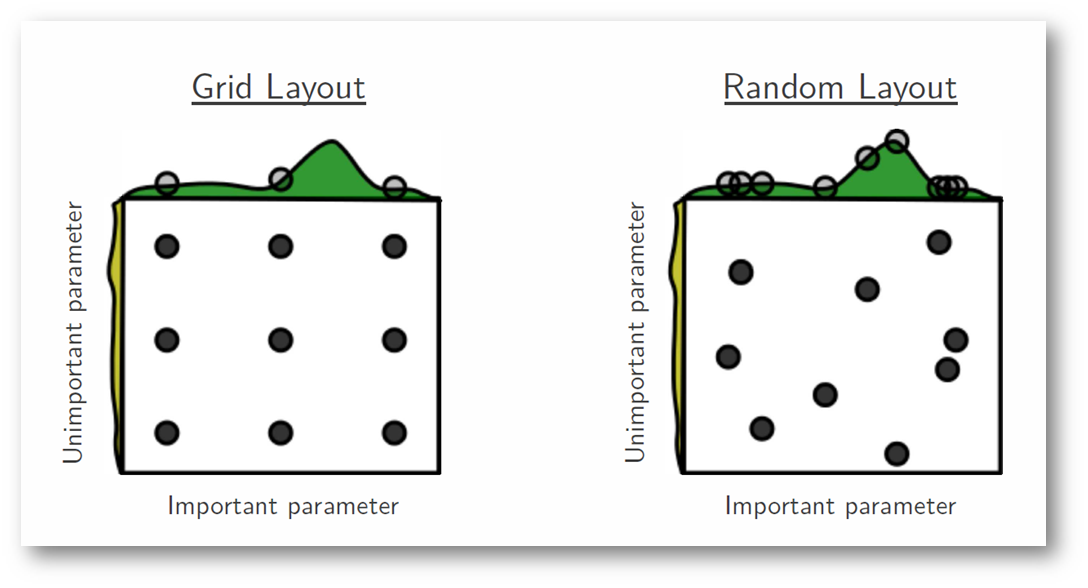
\includegraphics[scale=0.25]{09_evaluation/02_img/grid_random_search}
	\end{figure}
\end{frame}


% Subsection: Bias and Variance
% --------------------------------------------------------------------------------------------------------
\subsection{Bias and Variance}


% Bias and Variance
\begin{frame}{Bias and Variance}{}
	\begin{figure}
		\centering
		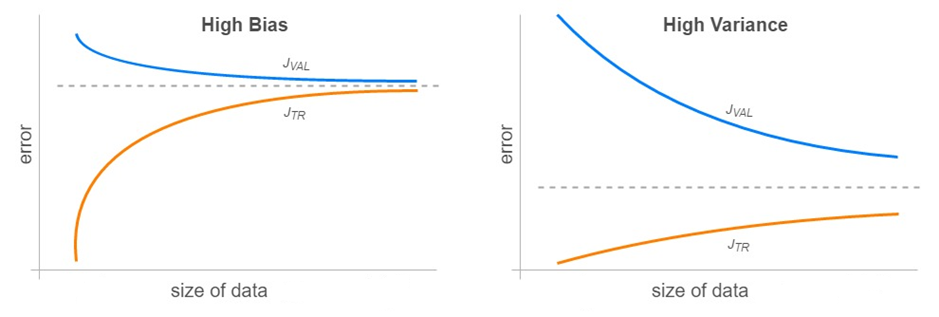
\includegraphics[scale=0.55]{09_evaluation/02_img/bias_variance}
	\end{figure}
\end{frame}


% Underfitting and Overfitting
\begin{frame}[plain]{}{}
	\bubble{1}{5}{
		\footnotesize Use early stopping!
	}
	\begin{figure}
		\centering
		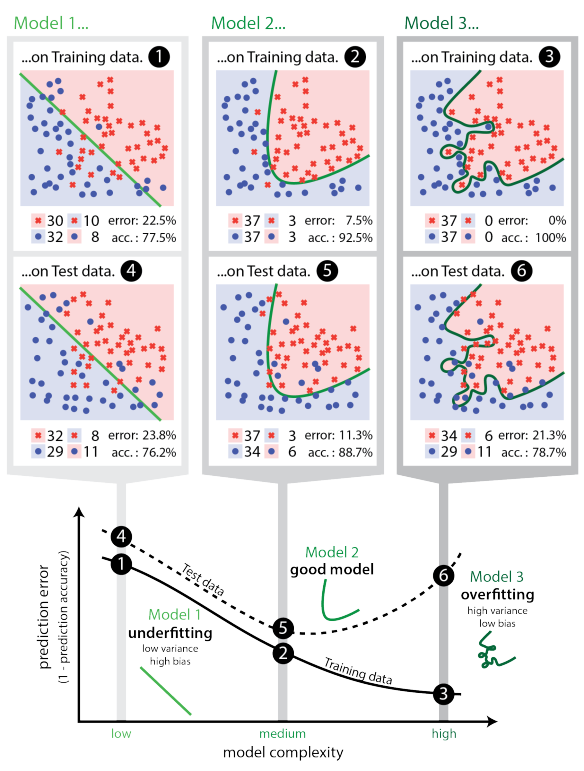
\includegraphics[scale=1.3]{09_evaluation/02_img/under_overfitting}
	\end{figure}
\end{frame}


% Section: Wrap-Up
%______________________________________________________________________
\section{Wrap-Up}
\makedivider{Wrap-Up}

% Subsection: Summary
% --------------------------------------------------------------------------------------------------------
\subsection{Summary}

% Summary
\begin{frame}{Summary}{}
	\begin{itemize}
		\item \textbf{Out-of-sample testing:} Split data into \texttt{train}, \texttt{dev} and \texttt{test} sets
		\item Cross-validation makes \textbf{maximum use of the data}
		\item Confusion matrices reveal \textbf{which classes are frequently confused}
		\item Precision, recall and F1 are \textbf{more robust w.\,r.\,t. imbalanced data sets}
		\item ROC curves are used for the evaluation of rankers
		\item Different classifiers can be optimal assuming a different cost model
		\item Hyper-parameters are optimized using \textbf{grid search} or \textbf{random search}
		\item Keep the \textbf{bias-variance trade-off} in mind!
	\end{itemize}
\end{frame}


% Subsection: Self-Test Questions
% --------------------------------------------------------------------------------------------------------
\subsection{Self-Test Questions}

% Self-Test Questions
\begin{frame}{Self-Test Questions}{}\important
	\begin{enumerate}
		\item Why should you split the data into \texttt{train}, \texttt{dev} and \texttt{test} sets?
		\item You perform 10-fold cross validation. How many models do you have to learn? Which one do you use in production?
		\item What is the problem with accuracy?
		\item Why do we apply the harmonic mean to compute the F1 score?
		\item Your model gets an AUC value of 0. What does this mean?
		\item Random search is usually preferred to optimize hyper-parameters. Why?
		\item Your model does not perform well due to its high bias.
			Your boss suggests adding more training data. How would you respond?
	\end{enumerate}
\end{frame}


% Subsection: Lecture Outlook
% --------------------------------------------------------------------------------------------------------
\subsection{Lecture Outlook}

\begin{frame}{What's next...?}{}
	\makeoverview{8}
\end{frame}


% Subsection: Recommended Literature and further Reading
% --------------------------------------------------------------------------------------------------------
\subsection{Recommended Literature and further Reading}

% Literature
%______________________________________________________________________
\begin{frame}[allowframebreaks]{Recommended Literature and further Reading}{}
	\footnotesize
	\begin{thebibliography}{2}
		\literature{book}{Mitchell.1997}{[1] Machine Learning}
			{Tom Mitchell. McGraw-Hill Science. 1997.}{$\rightarrow$ \href{
				https://www.cs.ubbcluj.ro/~gabis/ml/ml-books/McGrawHill\%20-\%20Machine\%20Learning\%20-Tom\%20Mitchell.pdf
			}{\linkstyle{Link}}, cf. chapter 5}
	\end{thebibliography}
\end{frame}


% Subsection: Meme of the Day
% --------------------------------------------------------------------------------------------------------
\subsection{Meme of the Day}

% Meme of the Day
\begin{frame}{Meme of the Day}{}
	\begin{figure}
		
\includegraphics[scale=0.4]{09_evaluation/02_img/meme_of_the_day}
	\end{figure}
\end{frame}


% Thank you
%______________________________________________________________________
\makethanks

\end{document}